\chapter{Introduction}
\paragraph{Manual Overview}
\paragraph*{
This is an Operation Manual for the Kodiak Saw (BPS NNN) revised control system programming. Each chapter topic covers one operator screen, along with related controls and indicators. The following format is used for indicating tips \textbf{\LARGE ( \textcolor{blue}{i} )} and cautionary notes \textbf{{\LARGE ( \textcolor{red}{!} )}} where necessary. As an example, the figure below shows the Main Operator Screen. Details will include items of interest, such as control items and information areas, as well as status indicators.
}
\begin{figure}
		\centering
		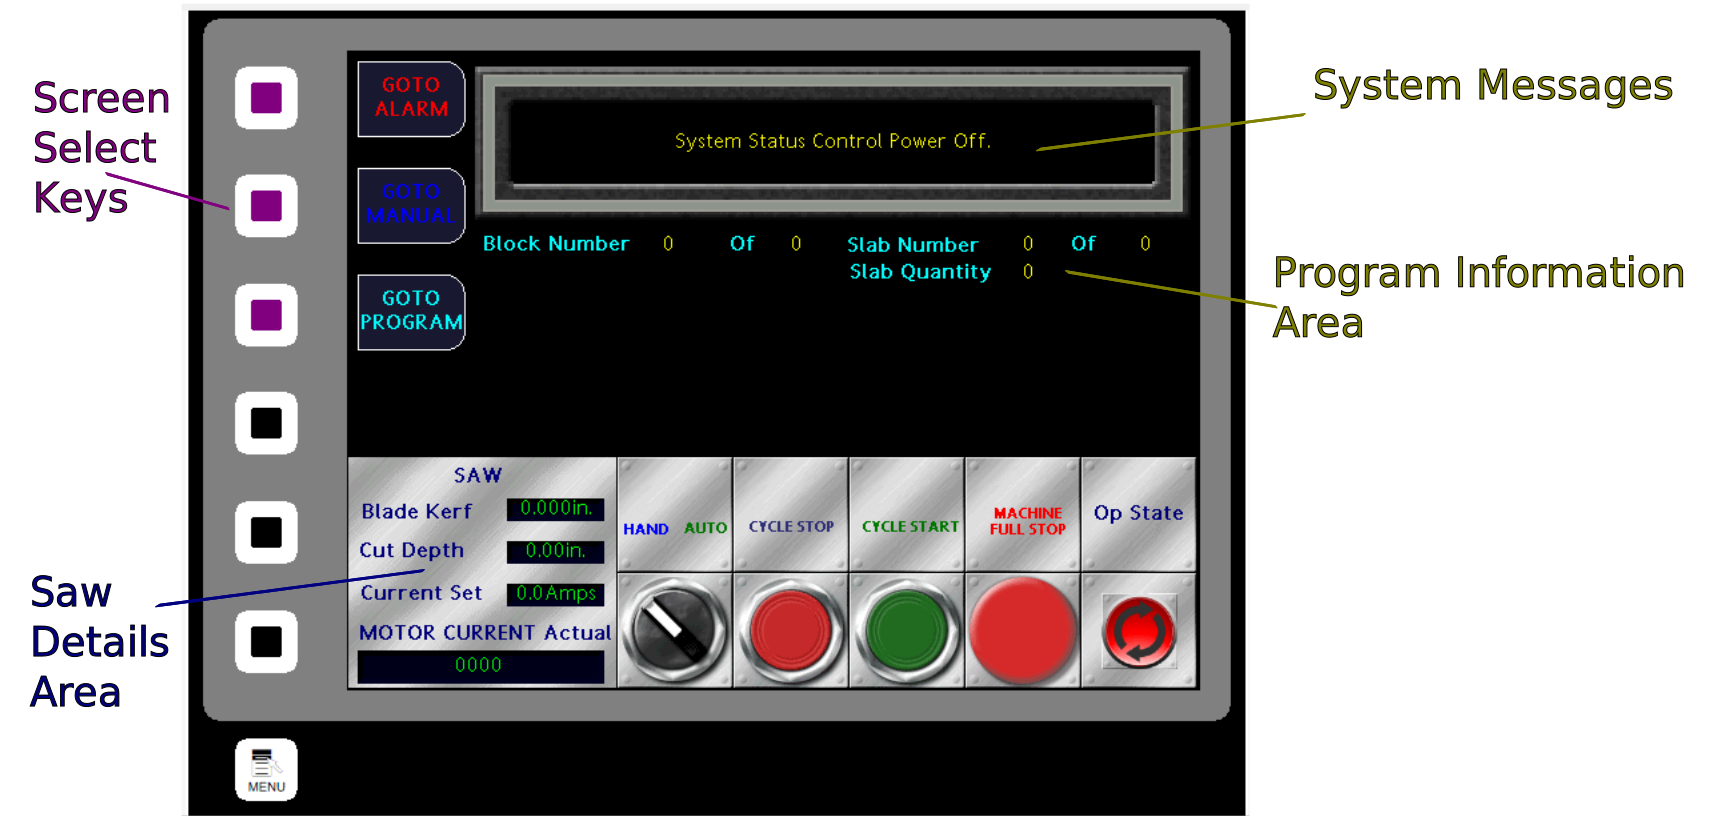
\includegraphics[width=0.7\linewidth]{screen-captures/main-screen}
		\caption{Main Screen}
		\label{fig:main-screen}
\end{figure}

